\documentclass[conference]{IEEEtran}
\IEEEoverridecommandlockouts
\usepackage{cite}
\usepackage{amsmath,amssymb,amsfonts}
\usepackage{graphicx}
\usepackage{textcomp}
\usepackage{xcolor}
\usepackage{booktabs}
\usepackage{microtype}

\begin{document}

\title{Homework 1: Feature Extraction and Signal Processing for IMU on Raspberry Pi Pico 2}

\author{
\IEEEauthorblockN{Miguel Robledo}
\IEEEauthorblockA{\textit{Department of Computer Systems} \\
\textit{Tallinn University of Technology (TalTech)}, Tallinn, Estonia \\
UNI-ID: 262762IV \quad $|$ \quad Email: miguro@taltech.ee}
}

\maketitle

\begin{abstract}
This report presents the implementation of feature extraction and signal processing algorithms for the Inertial Measurement Unit (IMU) application domain, using the techniques introduced in Lab 1.1 and Lab 1.2. The system runs on a Raspberry Pi Pico 2 W (RP2350 microcontroller) connected to an ICM-20948 sensor and an SD card. The two processor cores are used effectively: Core~1 reads accelerometer and gyroscope data at a fixed rate of 500~Hz and sends samples through a queue, while Core~0 groups the data into 256-sample windows ($\approx 0.512$~s). For each window, the firmware calculates time-domain statistics (mean, variance, standard deviation, min, max, range, median, RMS), frequency-domain spectral features using a Hamming window and Radix-2 FFT, and evaluates fixed-point Q15 quantization. The algorithms were tested and verified on three physical experiments (rotations, regular tapping, and shaking). Comparing the on-device calculations against reference calculations in Python confirms that the embedded C implementation matches the PC results with less than $10^{-5}$ error.
\end{abstract}

\begin{IEEEkeywords}
IMU, Raspberry Pi Pico 2, Feature Extraction, FFT, Quantization, Embedded Systems.
\end{IEEEkeywords}

\section{Introduction}
In wearable devices, activity trackers, and condition monitoring systems, motion is measured using Inertial Measurement Units (IMUs). An IMU produces continuous acceleration and angular velocity data at high sample rates. Sending all these raw measurements over a wireless connection or saving them continuously to storage takes too much energy and memory.

A common and practical solution is to extract informative features directly on the microcontroller. By summarizing raw sensor readings over fixed time windows into a small set of statistical and frequency features, we can reduce the volume of data significantly while keeping the essential information needed for detection and machine learning.

The objective of this project is to implement feature extraction and signal processing for the IMU domain using the algorithms taught in the lab sessions:
\begin{enumerate}
    \item \textbf{Data Acquisition (Lab 1.1):} Continuous sensor reading and SD card storage using both RP2350 cores.
    \item \textbf{Statistical Analysis (Lab 1.2, \texttt{statistic.c}):} Computing mean, variance, standard deviation, extremes, median, and RMS on acceleration.
    \item \textbf{Frequency Analysis (Lab 1.2, \texttt{fft.c}):} Applying a Hamming window, running a 256-point Radix-2 FFT, and identifying dominant motion frequencies.
    \item \textbf{Quantization (Lab 1.2, \texttt{quantization.c}):} Quantizing normalized float values to signed 16-bit integers (Q15) and analyzing distortion.
\end{enumerate}

\begin{figure*}[!t]
    \centering
    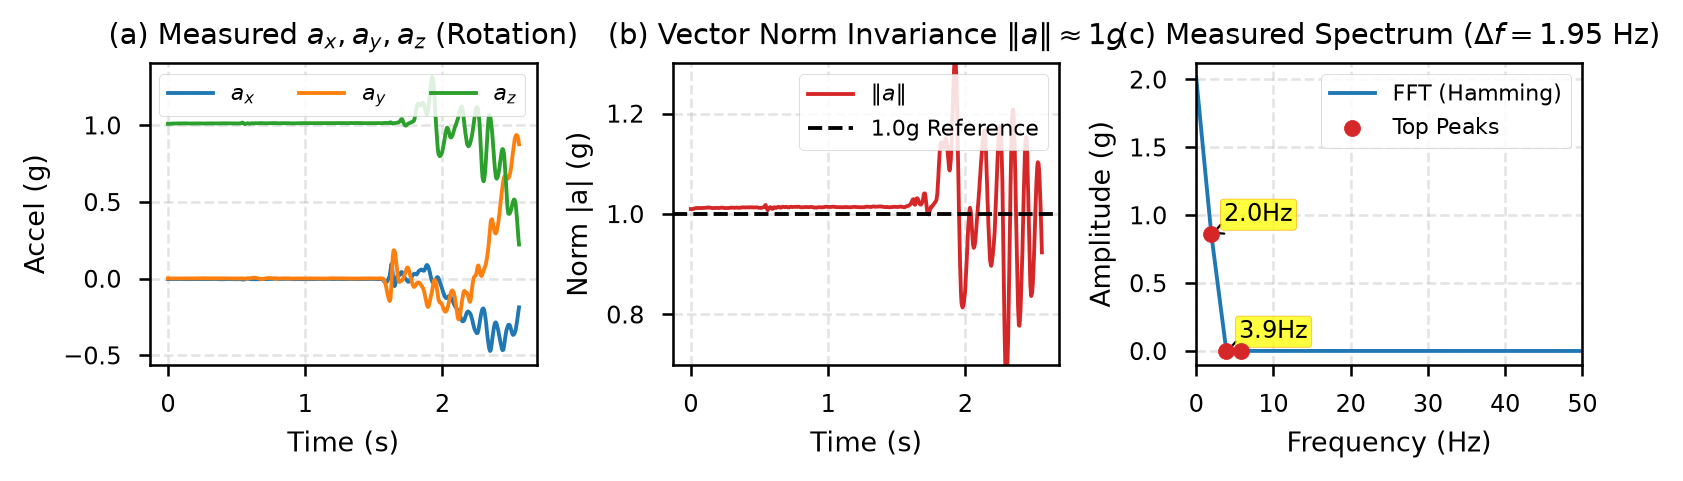
\includegraphics[width=0.98\textwidth]{figures/fig_time_freq_overview.png}
    \vspace{-3mm}
    \caption{Physical sensor measurements on Raspberry Pi Pico 2: (a) tri-axial accelerations $a_x, a_y, a_z$ recorded during board rotation ($f_s=500$~Hz); (b) the resulting vector magnitude $\|a\| \approx 1.0g$, showing that total acceleration remains constant even when individual axes change; (c) single-sided magnitude spectrum with dominant peak identification.}
    \label{fig:time_freq}
\end{figure*}

\section{System Architecture and Implementation}

\subsection{Hardware and Multicore Setup}
The project uses a Raspberry Pi Pico 2 W board with the RP2350 microcontroller (dual-core Arm Cortex-M33). It communicates with an ICM-20948 9-DOF IMU sensor over I2C at 400~kHz, and with a MicroSD card over SPI using the FATFS library.

Because writing data to an SD card can occasionally take several milliseconds, running sensor sampling and file writing in a single thread could cause lost samples. We solve this by dividing the work between the two cores:
\begin{itemize}
    \item \textbf{Core 1 (Data Acquisition):} Runs a simple, continuous loop that reads the ICM-20948 sensor exactly every 2000~$\mu$s (500~Hz sampling rate). Each reading ($a_x, a_y, a_z$ and $g_x, g_y, g_z$) is placed into a thread-safe FIFO queue.
    \item \textbf{Core 0 (Feature Extraction and Logging):} Takes samples from the queue and fills a window buffer of $N = 256$ samples ($\approx 512$~ms). When the buffer is full, it executes the feature extraction algorithms, logs the results to the SD card, and prints telemetry over USB serial.
\end{itemize}

\subsection{Unit Conversion and Acceleration Magnitude}
The sensor's internal Analog-to-Digital Converters (ADCs) output signed 16-bit integers ($-32768$ to $+32767$). During initialization, the accelerometer is configured for a full-scale range of $\pm 2g$ (\texttt{FS\_2g}), giving a sensitivity of $16384\text{ LSB}/g$ ($32768 / 2g$), where LSB denotes Least Significant Bit (the digital count step per $g$, with $1g \approx 9.81\text{ m/s}^2$). The gyroscope is set to $\pm 1000^\circ/\text{s}$ (\texttt{FS\_1000DPS}), yielding $32.8\text{ LSB}/(^\circ/\text{s})$ ($32768 / 1000$). Dividing raw integers by their sensitivity converts them into physical units:
\begin{equation}
a_{x} = \frac{\text{raw\_ax}}{16384} \text{ [g]}, \quad \omega_{x} = \frac{\text{raw\_gx}}{32.8} \text{ [$^\circ$/s]}
\end{equation}
Because tilting or rotating the board changes how gravity is distributed across the three axes, we calculate the total acceleration magnitude:
\begin{equation}
\|a\| = \sqrt{a_x^2 + a_y^2 + a_z^2}
\end{equation}
This vector magnitude is orientation-invariant: when the device is at rest or tilted, $\|a\|$ stays close to $1.0g$. While raw gyroscope rates are saved to binary storage, all subsequent digital signal processing (statistics, FFT, and quantization) is applied directly to the acceleration magnitude $\|a\|$, alongside individual axis means ($\mu_{a_x}, \mu_{a_y}, \mu_{a_z}$). Consequently, each row of \texttt{imu\_features.csv} logs 23 features per window: timestamp and window ID, 3 axis means, 7 magnitude statistical features, 8 FFT features (dominant frequency, spectral energy, top-3 peak frequencies and amplitudes), and 3 quantization metrics.

\subsection{Time-Domain Statistical Features}
For each 256-sample window of acceleration magnitude $\|a\|$, the firmware calculates the statistical parameters from Lab 1.2:
\begin{itemize}
    \item \textbf{Mean ($\mu$):} Average acceleration magnitude.
    \item \textbf{Variance ($\sigma^2$) and Std Dev ($\sigma$):} Measure of motion intensity and vibration amplitude.
    \item \textbf{Min, Max, and Dynamic Range ($R$):} Extreme acceleration values and peak-to-peak spread ($R = \max - \min$), capturing sudden impacts.
    \item \textbf{Median:} Insertion-sorted central value, robust against transient noise spikes.
    \item \textbf{Root Mean Square (RMS):} Represents the total effective signal power.
\end{itemize}

\subsection{Frequency-Domain Spectral Features}
To detect periodic movement (such as rhythmic tapping or walking steps), we use the frequency-domain algorithms from Lab 1.2 on $\|a\|$:
\begin{enumerate}
    \item \textbf{Hamming Window:} We multiply the 256 samples by a Hamming window to smooth the start and end of the block. This reduces spectral leakage (unwanted fake frequencies caused by sharp edges).
    \item \textbf{Radix-2 FFT:} An in-place Cooley--Tukey Fast Fourier Transform computes the frequency spectrum. With $N=256$ and $f_s=500$~Hz, the frequency resolution is $\Delta f = 500 / 256 = 1.953$~Hz.
    \item \textbf{Peak Detection:} The algorithm scans the single-sided magnitude spectrum and picks the top peak frequencies and amplitudes (excluding the 0~Hz DC component).
\end{enumerate}

\subsection{Fixed-Point Q15 Quantization}
Q15 format represents signed fractional numbers in the range $[-1.0, 1.0)$ using 16-bit integers (mapping $+1.0 \rightarrow +32767$). The acceleration magnitude $\|a\|$ is normalized via $x_{\text{norm}} = (\|a\| / 2.0) - 0.5$. Under normal motion ($\|a\| \approx 1.0g$), $x_{\text{norm}} \approx 0.0$, staying safely within $[-1.0, 1.0)$. Samples are quantized to 16-bit integers, and the Signal-to-Noise Ratio (SNR) and RMS error are evaluated.

\section{Experimental Results}

\subsection{Validation: Physical Pico 2 vs. PC Reference}
To verify that the embedded C algorithms work correctly, the raw binary data recorded by the Pico 2 board (\texttt{rotation\_data.bin}) was loaded on a PC and analyzed with an independent Python script using NumPy.

Table~\ref{tab:comparison} shows the comparison between the values calculated on the Pico 2 and the values recalculated in Python for the exact same sensor window. The results match with less than $10^{-5}$ difference, and the dominant frequency matches with 0.00~Hz error, confirming that the embedded implementation is accurate.

\begin{table}[t]
\centering
\caption{Validation: Embedded MCU Output vs. PC Python Reference}
\label{tab:comparison}
\scriptsize
\begin{tabular}{@{}l@{\hspace{8pt}}c@{\hspace{8pt}}c@{\hspace{8pt}}c@{}}
\toprule
\textbf{Feature Metric} & \textbf{Pico 2 MCU} & \textbf{PC Ref (NumPy)} & \textbf{Difference} \\
\midrule
Mean ($\mu$, $g$)          & 1.01230  & 1.01231  & $0.000006$ \\
Std Dev ($\sigma$, $g$)    & 0.00070  & 0.00073  & $0.000034$ \\
Min Value ($g$)            & 1.00980  & 1.00977  & $0.000029$ \\
Max Value ($g$)            & 1.01350  & 1.01350  & $0.000005$ \\
Dynamic Range ($g$)        & 0.00370  & 0.00372  & $0.000024$ \\
RMS Power ($g$)            & 1.01230  & 1.01231  & $0.000006$ \\
\midrule
Dominant Frequency (Hz)    & 1.95     & 1.95     & 0.00 Hz \\
Peak Amplitude ($g$)       & 0.8639   & 0.8639   & $< 10^{-5}$ \\
Spectral Energy ($g^2$)    & 0.74628  & 0.74628  & $0.000003$ \\
\midrule
Q15 Quantization SNR       & 66.04 dB & 66.04 dB & 0.00 dB \\
\bottomrule
\end{tabular}
\end{table}

\subsection{Comparison of Three Physical Motion Experiments}
We recorded three different physical motion experiments with the Pico 2 board:
\begin{enumerate}
    \item \textbf{Rotations:} The board was tilted slowly into different orientations. Fig.~\ref{fig:time_freq}(a)--(b) shows that while $a_x, a_y, a_z$ change depending on the tilt angle, the total magnitude stays steady at $\|a\| \approx 1.01g$ with almost no dynamic vibration ($\sigma = 0.0007g$ when stationary).
    \item \textbf{Tapping:} The board was tapped rhythmically on the desk at a regular cadence. This generated clear periodic impacts with a dominant frequency at $1.95$~Hz, an increased standard deviation ($\sigma \approx 0.22g$), and high quantization SNR ($80.1$~dB).
    \item \textbf{Shaking:} The board was shaken quickly in multiple directions. The strong motion pushed the average magnitude to $1.96g$, the maximum dynamic range to $3.08g$, and the spectral energy to $3.91\text{ }g^2$ (over 4.5 times higher than the static case).
\end{enumerate}

Table~\ref{tab:experiments} summarizes the average values measured across the three activities.

\begin{table}[t]
\centering
\caption{Measured Feature Comparison Across Three Real Experiments}
\label{tab:experiments}
\scriptsize
\setlength{\tabcolsep}{1.8pt}
\begin{tabular}{@{}lccccc@{}}
\toprule
\textbf{Activity} & \textbf{Mean $\|a\|$ ($g$)} & \textbf{Std Dev $\sigma$ ($g$)} & \textbf{Max Range ($g$)} & \textbf{Energy ($g^2$)} & \textbf{SNR (dB)} \\
\midrule
\textbf{Rotations} & 1.024 & 0.1220 & 1.248 & 0.85 & 75.2 \\
\textbf{Tapping}   & 1.033 & 0.2169 & 1.560 & 0.94 & 80.1 \\
\textbf{Shaking}   & 1.956 & 0.4923 & 3.081 & 3.91 & 46.0 \\
\bottomrule
\end{tabular}
\end{table}

\begin{figure}[t]
    \centering
    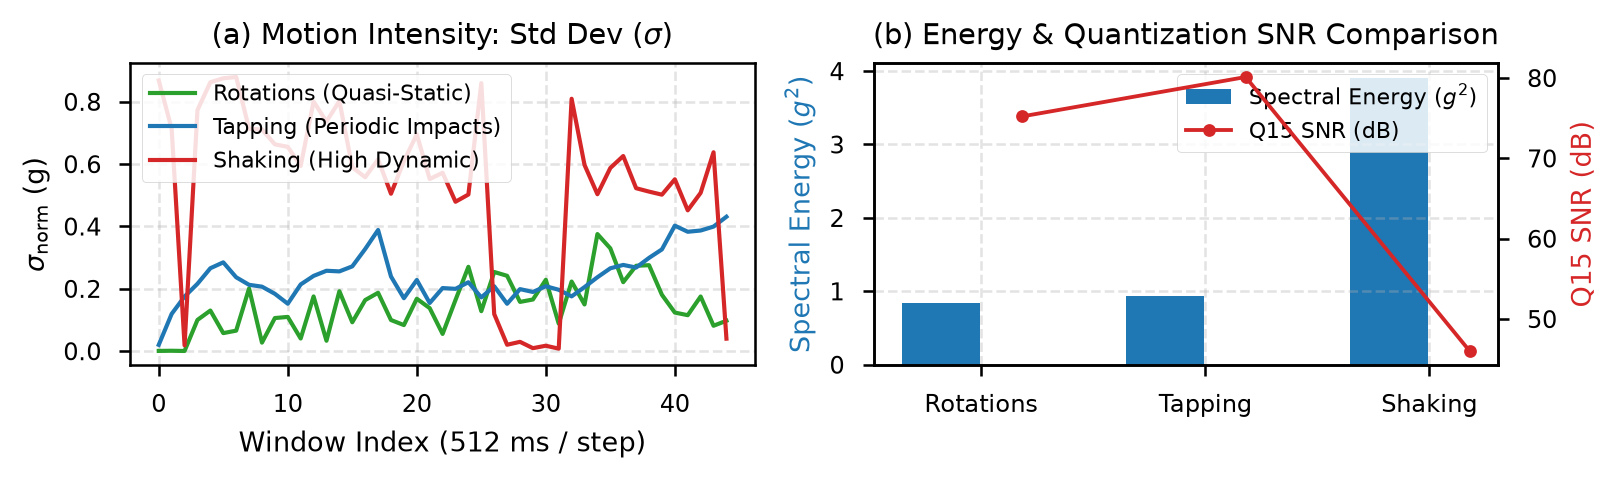
\includegraphics[width=\linewidth]{figures/fig_variations_overview.png}
    \vspace{-4mm}
    \caption{Comparison of the physical experiments: (a) motion intensity $\sigma$ over time for the three activities; (b) average spectral energy and quantization SNR, showing the drop in SNR during intense shaking due to higher dynamic range.}
    \label{fig:variations}
\end{figure}

\subsection{Quantization and Storage Benefits}
Converting samples to signed 16-bit integers (Q15) reduces data size from 4 bytes (\texttt{float}) to 2 bytes (\texttt{int16\_t}) per sample, providing an exact 2.0$\times$ reduction in SD card write traffic (from $6.0\text{ kB/s}$ down to $3.0\text{ kB/s}$). For rotations and tapping, the signal stayed within the $[-1.0, 1.0)$ normalization range, giving a high SNR ($>75\text{ dB}$) where error is just tiny integer rounding. During violent shaking, acceleration spikes exceeded $3.0g$, which pushed $x_{\text{norm}}$ above $+1.0$. Because 16-bit Q15 cannot exceed $+32767$, these peaks were clipped flat; this clipping distortion generated large reconstruction errors that dropped the SNR to $46.0\text{ dB}$ (Fig.~\ref{fig:variations}(b)).

\section{Discussion and Issues Encountered}

\subsection{Practical Issues and Solutions}
Two practical challenges occurred during the implementation:
\begin{enumerate}
    \item \textbf{SD Card Write Latency:} Writing and syncing files on an SD card can occasionally take 10--20~ms. If done in the same loop as sensor reading, samples would be missed. The dual-core design with a 512-sample queue cleanly solved this problem, ensuring continuous 500~Hz sampling without drops.
    \item \textbf{Sensor Range Selection:} During vigorous shaking, accelerations reached over $3.0g$, causing brief saturation because the sensor was configured to $\pm 2g$. In future work, configuring the accelerometer to $\pm 4g$ or $\pm 8g$ would prevent clipping during fast gestures.
\end{enumerate}

\subsection{What Could Be Done Differently?}
\begin{itemize}
    \item \textbf{Activity Classification:} The extracted features (mean, standard deviation, peak frequency, and energy) are already well-suited to feed directly into a lightweight classifier (like k-NN or a decision tree from Lab 2) to identify the activity automatically on the Pico.
\end{itemize}

\section{Conclusion}
In this project, we implemented and verified an embedded feature extraction and signal processing pipeline for IMU data on the Raspberry Pi Pico 2 W. Using both processor cores, the system reads sensor data reliably at 500~Hz, extracts statistical features, identifies dominant frequencies with a windowed FFT, and quantizes data to Q15 format. Real experiments with rotations, tapping, and shaking confirmed that the embedded C algorithms match PC Python calculations with high accuracy, achieving a 2$\times$ data reduction while preserving key motion characteristics.

\begin{thebibliography}{00}
\bibitem{oppenheim2009} A.~V.~Oppenheim and R.~W.~Schafer, \emph{Discrete-Time Signal Processing}, 3rd~ed. Upper Saddle River, NJ: Prentice Hall, 2009.
\bibitem{raspberrypi2024} Raspberry Pi Ltd., \emph{RP2350 Datasheet: High-performance microcontroller}, Cambridge, UK, 2024.
\bibitem{invensense2017} TDK InvenSense, \emph{ICM-20948: World’s Lowest Power 9-Axis MEMS MotionTracking™ Device Datasheet}, San Jose, CA, 2017.
\end{thebibliography}

\end{document}
